\chapter{Baseline}
\label{chap:Baseline}
This chapter introduces the baseline architecture, which processes an evolving graph. First off, we will go through an overview of the task and a rather ``textual`` description of the model. \\

Then, the baseline model will be described in a more precise way as well as a schematic visualization of the operations that are performed.

\section{Overview}
The baseline architecture deals with the problem of processing a single graph, evolving over time. This graph that will be fed to the downstream model is represented by a series of states.\\

In our case the input entities of interest in our graph are admissions, and the simplest way to predict the diagnoses at discharge of a given input admission is to only consider its events over time as our evolving graph and not directly considering the information from other admission entities. That is, in this baseline approach, we do not consider a knowledge graph linking admissions together within a complex structure, but rather admissions as individual evolving graphs consisted of chunk and event entities. \\

\begin{wrapfigure}{l}{0.5\textwidth}
 \centering
 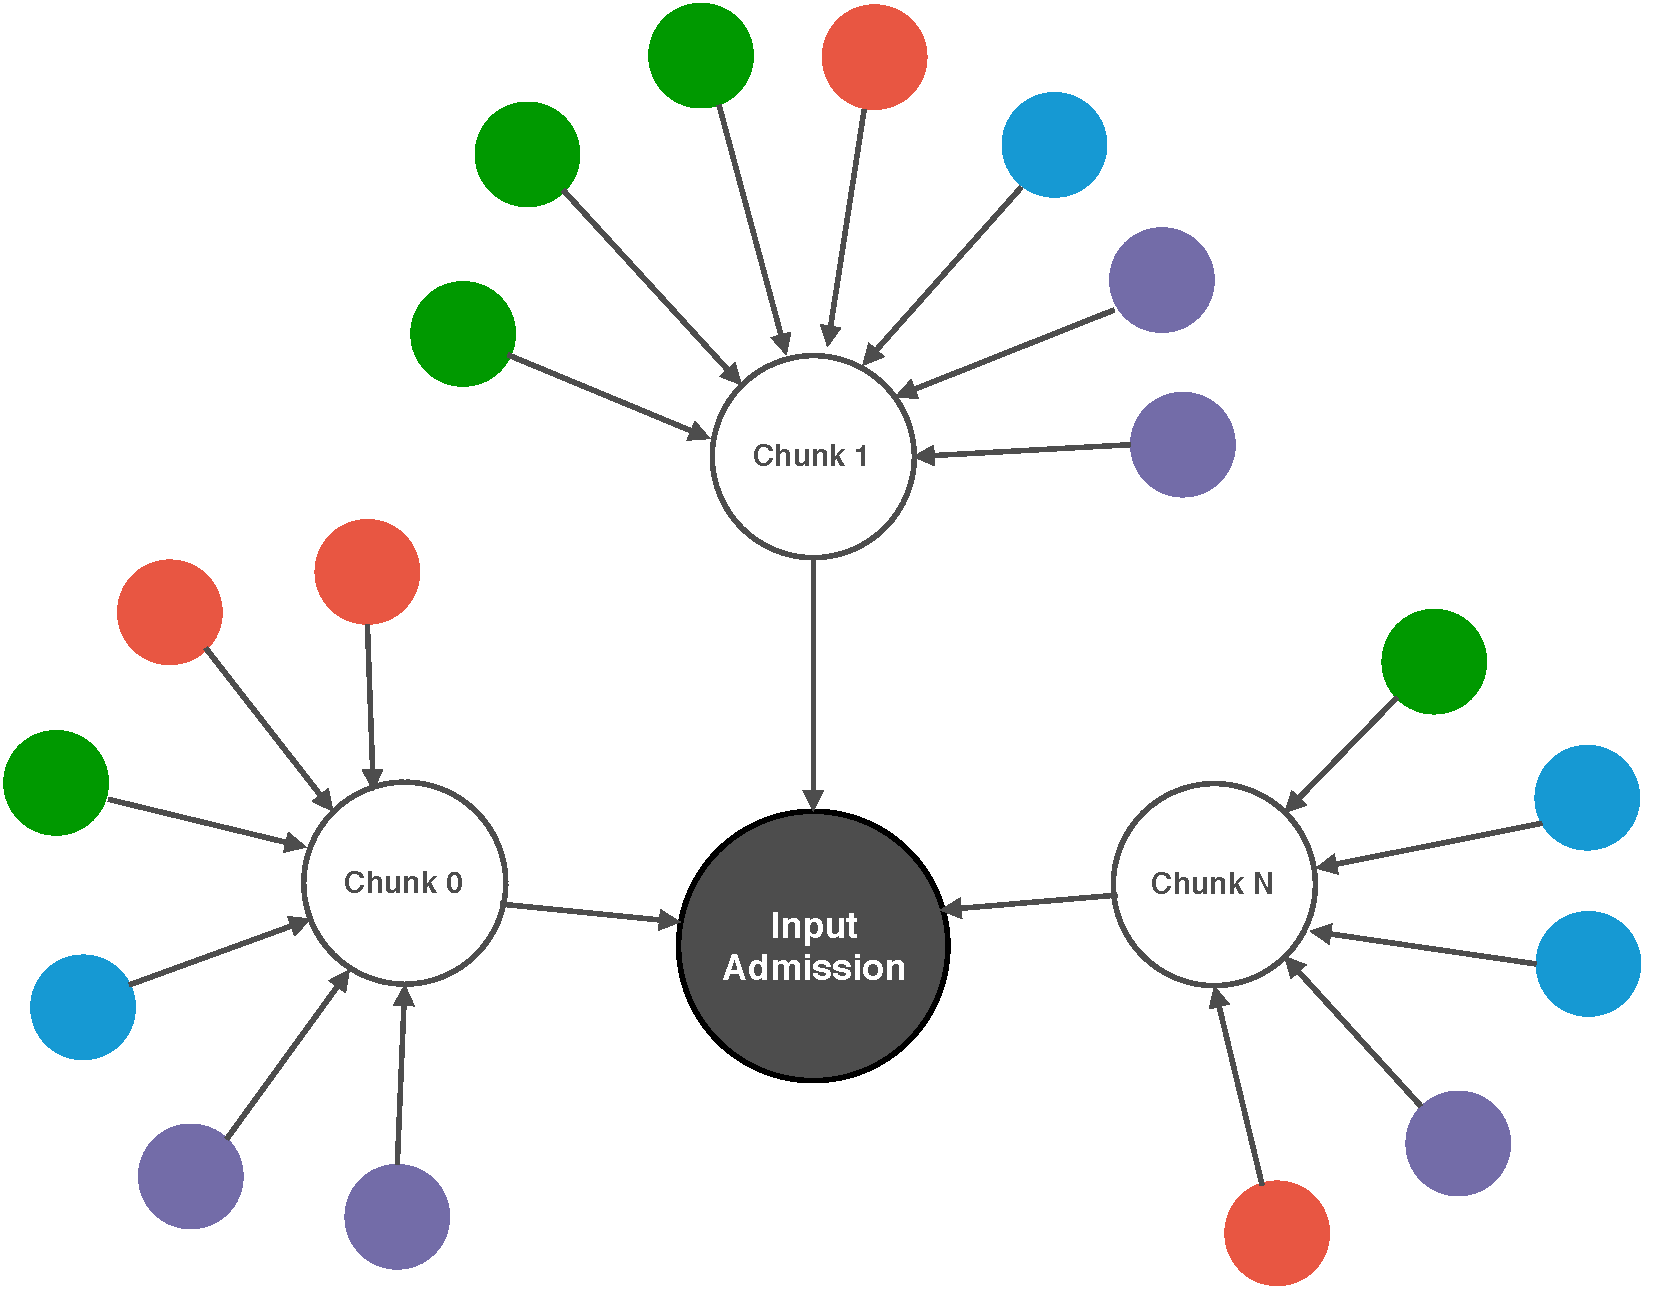
\includegraphics[width=.8\linewidth]{figures/single-adm-graph.pdf}
 \captionsetup{width=.8\linewidth}
 \caption{Example admission (\textit{without} zero padding), where chunk entities have a natural ordering and event entities do not.}
 \label{fig:single-adm-graph}
\end{wrapfigure}

Such a graph can be represented in a compact form as shown in the figure~\ref{fig:single-adm-graph}, the colored entities refer to particular events during the admission timeline, associated to a given chunk depending on the chart time. This admission has a set of diagnoses at discharge and we are looking for an architecture that would enable us to capture the dynamic behavior as well as make sense of the different events. \\

Therefore, it is natural that we base our research and baseline architecture on a Recurrent Neural Network to deal with the different chunks or states of the graph, this type of architecture allowing exploiting temporal dynamic behavior for sequence. Consequently, we need to input an embedded representation of the graph state at every time step $T$ in our Recurrent Neural Network. That is, we need to \textit{map} our graph state into a finite D-dimensional vector (where D is a hyper-parameter to be chosen appropriately) that will enable us to train the model end-to-end. Indeed, as opposed to older techniques that embed the graph in a separate task, making the back-propagation truncated between the RNN and the graph embedding algorithm, we want our architecture to be fully differentiable. \\

\section{Machine Learning Model}
Unlike performing machine learning over classical lattices (e.g. images), the neighboring entities or nodes (i.e. \textit{events}) to our graph states do not have a natural ordering. For this reason, owing to GraphSAGE~\cite{DBLP:journals/corr/HamiltonYL17}, we base our ``graph state embedder`` on aggregator functions for each entity type. These functions must operate over an unordered set of vectors and thus be invariant to permutations of its elements. \\

However, before discussing the aggregator functions in detail, the different events as well as their respective value should be ``translated`` in vector forms. As an illustration, let's consider the following event from the \textbf{Prescriptions table}:

\begin{equation*}
 e^{prescription} = (\mbox{Warfarin}, 5)
\end{equation*}

This tuple represents an entity of the type \emph{prescription event}, where the patient took 5 units of Warfarin. From there, we create a \textbf{prescription embedding matrix} that maps from ``Warfarin`` to a $n$-dimensional vector, where $n$ is a hyper-parameter to be tuned carefully. Finally, this \textbf{prescription embedding matrix}, $M\in\mathbb{R}^{P \times n}$ where $P$ represents the number of prescriptions (4'465 in our case), is initialized with zero-vectors. \\

At the beginning of the training procedure, each prescription event is mapped to its corresponding $n$-dimensional vector and concatenated to its associated value:

\begin{equation*}
\tilde{e}^{prescription} = [\bm{x}, 5]\mbox{, where }\bm{x}\in\mathbb{R}^n
\end{equation*}

At the end of this ``translation`` procedure, each prescription event entity is a $(n+1)$-dimensional vector that can be further processed. In a similar fashion, we create an embedding matrix for each event types, resulting in 5 different embedding matrices initialized with zero-vectors that will allow to ``translate`` every event entities in the evolving graph. \\

Hence, a chunk $i$ can be represented as a tensor of shape $5 \times K \times (n+1)$, resulting from the concatenation of the different event types. Thus, an admission can be seen as a series of chunks, leading to a tensor of shape $N \times 5 \times K \times (n+1)$ for each admission. \\

As mentioned previously, these aggregators should be invariant to permutations of the input, trainable and also have a high representational capacity. To this end, each \textit{aggregator} will first consist of a fully-connected network and followed by the aggregation function, we propose three candidates:

\paragraph{Max aggregator} The first nominee consists in element-wise max-pooling operation along the $K$ dimension. Namely, we have the following end-to-end aggregator:

\begin{equation}
 \label{eq:max_agg}
 \begin{aligned}
 AGG_m^{max} &= \max_{i \in \{0 \dots K\}} \sigma(\bm{W}\bm{\tilde{e}}_i^m + \bm{b})\mbox{, where }\bm{\tilde{e}}_i^m \in \mathbb{R}^{n+1} \\
 &= \max_{i \in \{0 \dots K\}} \bm{h}_i^m\mbox{, where }\bm{h}_i^m \in \mathbb{R}^{a}
 \end{aligned}
\end{equation}

Here $\max$ denotes the element-wise max operator along the $K$ dimension, $\sigma$ is a nonlinear activation function (e.g. ReLU) and $a$ is an arbitrary dimensionality that has to be manually tuned. Besides, $m$ represents the event type among laboratory measurements, input events (CV or MV), output events and prescriptions, while $\bm{W} \in \mathbb{R}^{a \times (n+1)}$ and $\bm{b} \in \mathbb{R}^a $ are parameters optimized during the back-propagation training. \\

All in all, for each event type $m$, the equation~\ref{eq:max_agg} maps each embeddings to a $a$-dimensional hidden representation $\bm{h}_i^m$ and then squashes the events of a similar type with the max operator.

\paragraph{Mean aggregator} This aggregator is very similar to the \textit{max aggregator} but performs a mean-pooling operation along the $K$ dimension:

\begin{equation}
 \label{eq:max_agg}
 \begin{aligned}
  AGG_m^{mean} 
   &= \underset{i \in \{0 \dots K\}}{\mbox{mean}} \sigma(\bm{W}\bm{\tilde{e}}_i^m + \bm{b})\mbox{, where }\bm{\tilde{e}}_i^m \in \mathbb{R}^{n+1} \\
   &= \underset{i \in \{0 \dots K\}}{\mbox{mean}} \bm{h}_i^m\mbox{, where }\bm{h}_i^m \in \mathbb{R}^{a}
 \end{aligned}
\end{equation}

\paragraph{Sum aggregator} Our final candidate looks like the two previous ones, by replacing the element-wise operator with a sum operation:

\begin{equation}
\label{eq:max_agg}
 \begin{aligned}
 AGG_m^{sum} 
  &= \underset{i \in \{0 \dots K\}}{\mbox{sum}} \sigma(\bm{W}\bm{\tilde{e}}_i^m + \bm{b})\mbox{, where }\bm{\tilde{e}}_i^m \in \mathbb{R}^{n+1} \\
  &= \underset{i \in \{0 \dots K\}}{\mbox{sum}} \bm{h}_i^m\mbox{, where }\bm{h}_i^m \in \mathbb{R}^{a}
 \end{aligned}
\end{equation}

A visual explanation is available on the figure~\ref{fig:agg-example}. In essence, it is important to note that all of these aggregators are both symmetric and trainable. Once stacked, the output of these aggregators is a tensor of shape $N \times 5 \times a$ that we further reshape and concatenate to $N \times 5a$ in order to be fed to our downstream Recurrent Neural Network. Thus, referring to the previous section, each $5a=D$ vector is our representation of the graph state at the time step $T$. \\

This Recurrent Neural Network outputs a vector of size $\bm{\tilde{h}} \in \mathbb{R}^{b}$ that is represented the embedding of our \textbf{evolving entity}. In our practical use-case to predict the ICD9 codes at discharge, we simply feed this vector into a fully-connected layer mapping to our \emph{50} classes.\\

More generally, this embedding algorithm followed by a Recurrent Neural Network is applicable to any arbitrary entity and we call it an \textbf{Evolving Entity Encoder}. We present the baseline model applied to our ``Healthcare Dataset`` but it generalizes easily to different graphs and structures, since it is independent of the number of neighbors.

\begin{figure}[h]
 \centering
 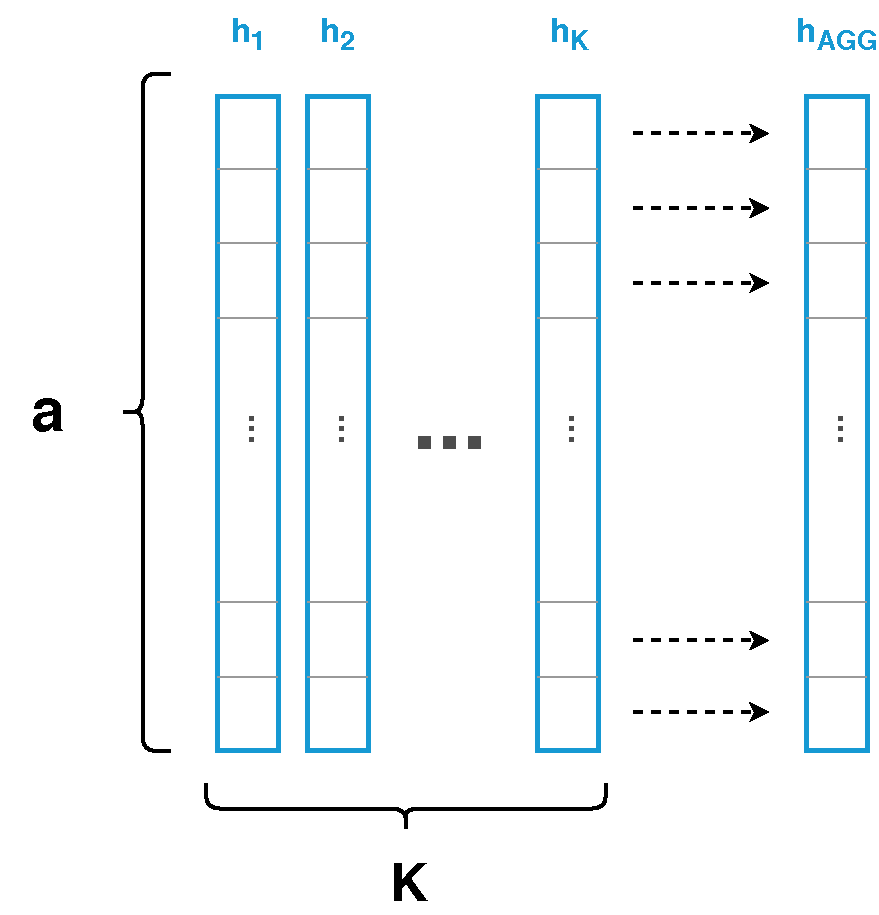
\includegraphics[width=0.35\textwidth]{figures/agg-example.pdf}
 \caption{An example of an aggregator on a certain event type (\textit{blue}), the dashed arrow represent the type of aggregating function (i.e. sum, mean, max) applied element-wise (row-by-row on the figure). The output is a vector $\bm{h}_{AGG} \in \mathbb{R}^{a}$.}
 \label{fig:agg-example}
\end{figure}

\newpage
\begin{landscape}
 \section{Schematic Visualization}
 To better understand how the baseline architecture works and generalizes to arbitrary graphs, we propose the following visualizations to the reader: \\
 
 \begin{figure}[H]
  \centering
  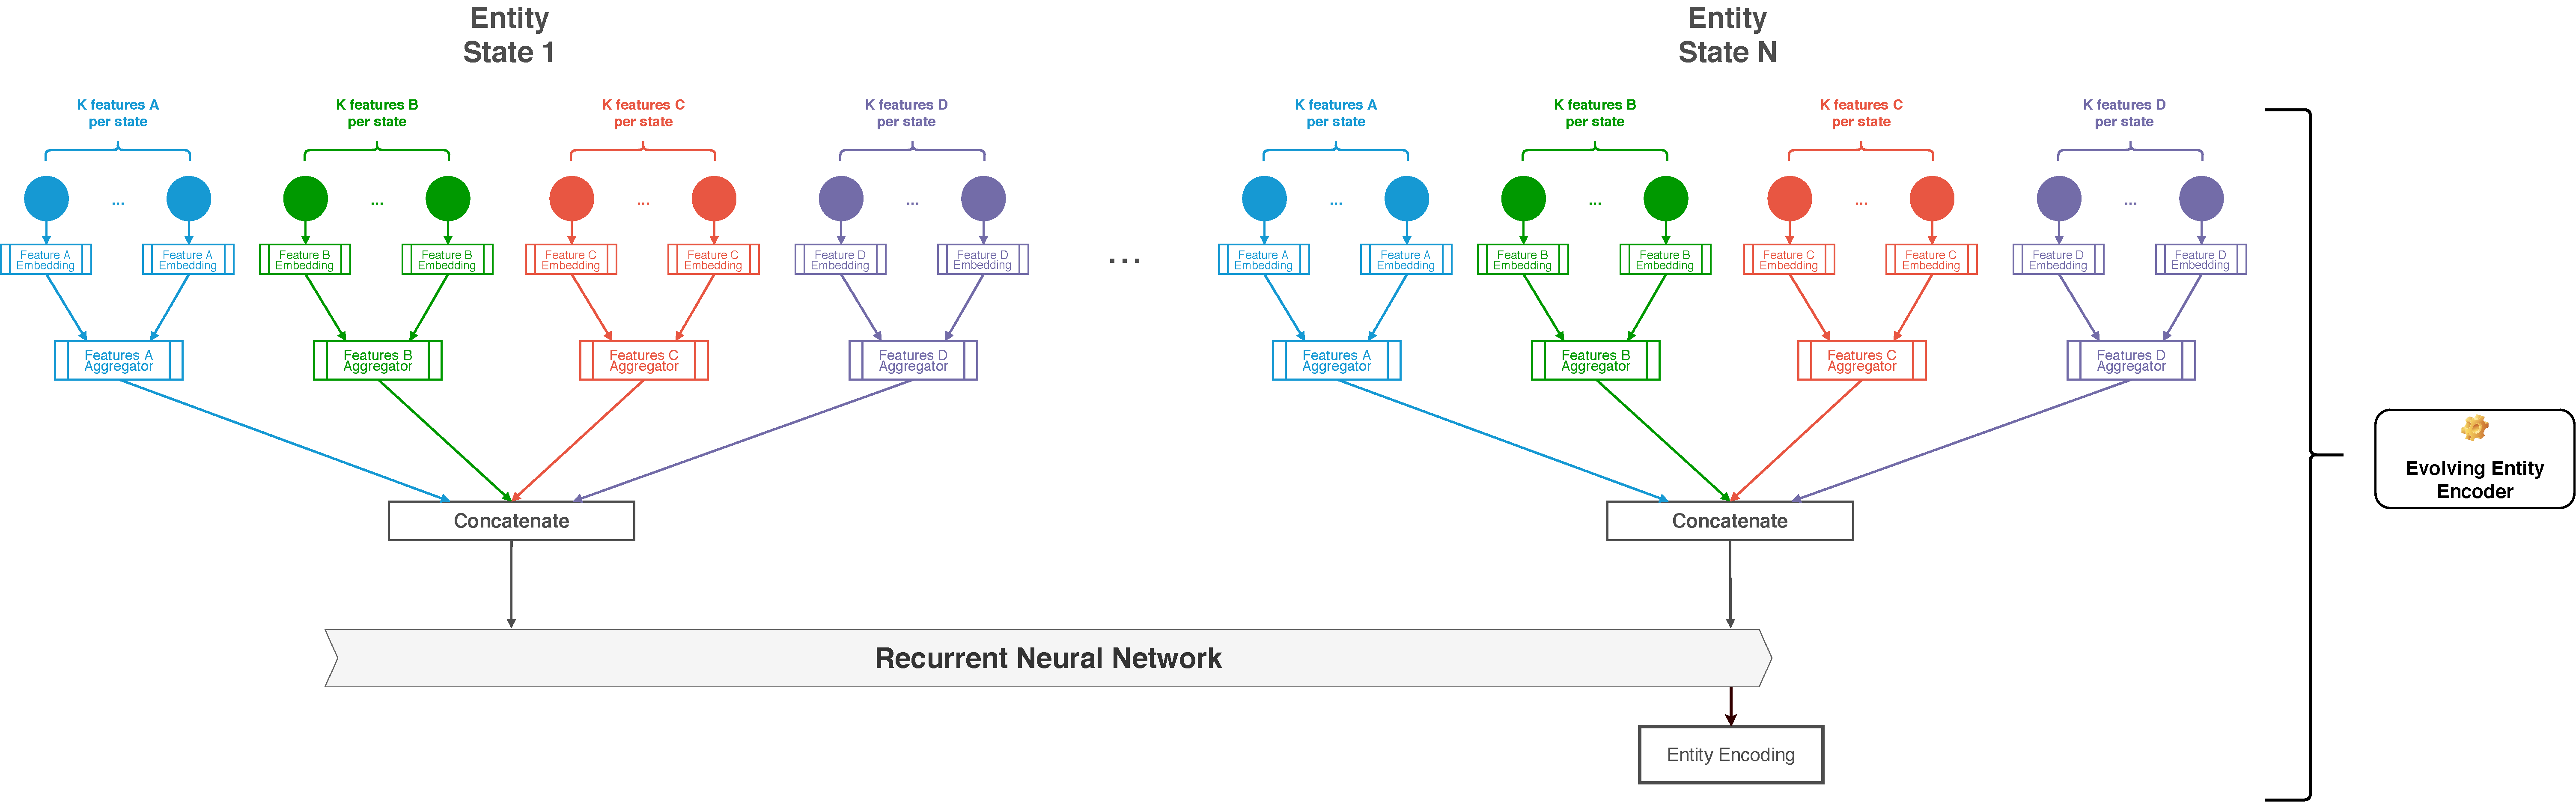
\includegraphics[width=\linewidth]{figures/encoder-general.pdf}
  
  \caption{Visualization of the \emph{Evolving Entity Encoder}, that passes each feature through their respective embedding, then aggregator and concatenate the results to be finally fed through the Recurrent Neural Network. This is application-agnostic and supports a varying number of features for each entity.}
 \end{figure}
\end{landscape}
\newpage
\begin{landscape}
\begin{figure}[H]
 \centering
 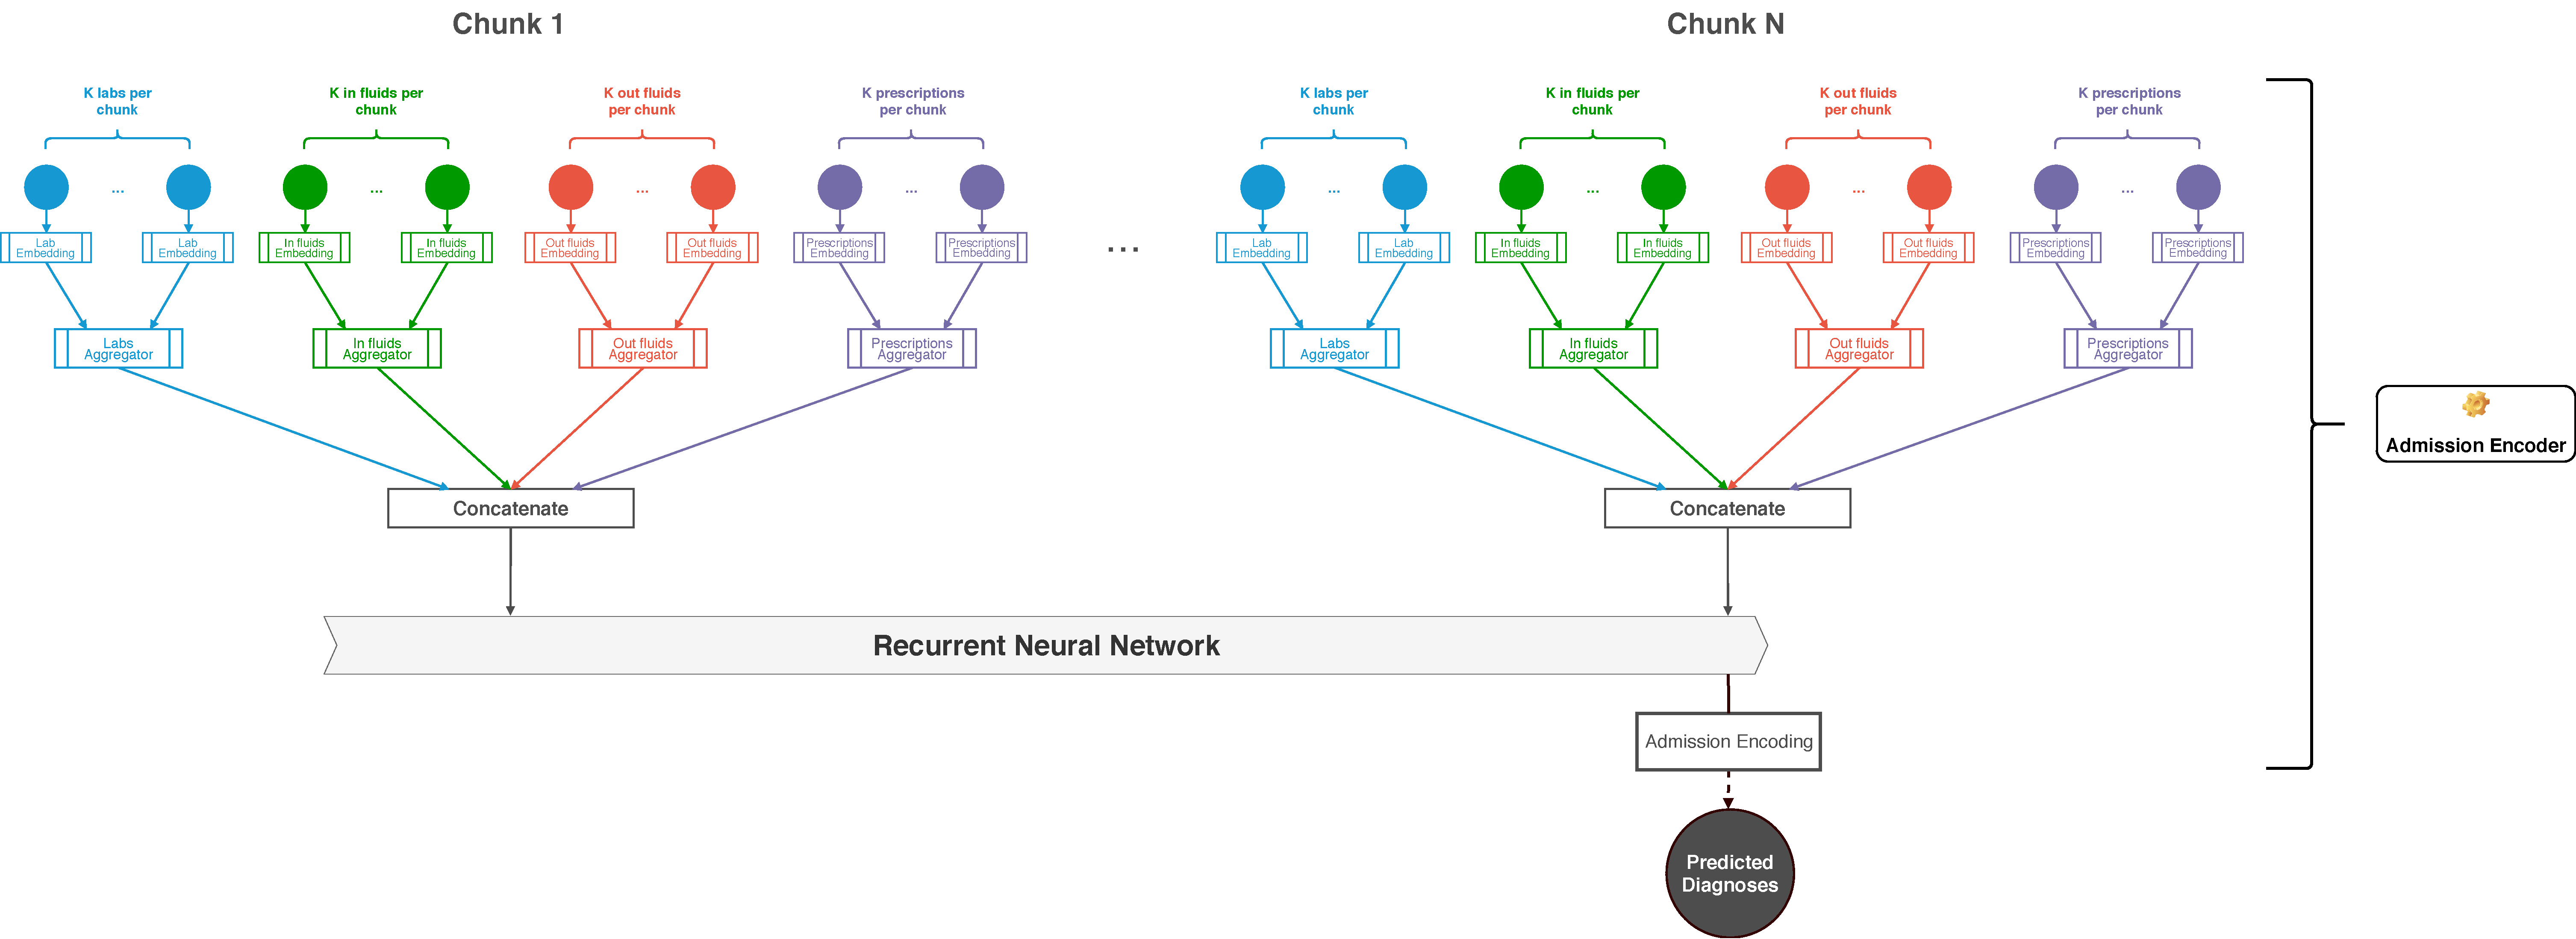
\includegraphics[width=\linewidth]{figures/encoder-healthcare.pdf}
 
 \caption{The \emph{Evolving Entity Encoder} applied to our use-case. Hence, we are encoding an admission that consists in an evolving patient state to finally predict the diagnoses at discharge with an additional fully-connected layer.}
\end{figure}
\end{landscape}